\documentclass[border=10pt]{standalone} 
\usepackage{tikz}

\begin{document}    

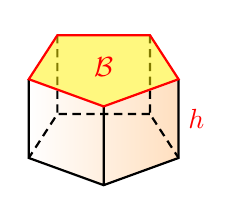
\begin{tikzpicture}
% fill/draw front part of cylinder
\fill[left color=orange!0, right color=orange!25] 
    (198:{1 and 0.5})
        -- ++(0,-1)
        -- ([shift={(down:1)}]270:{1 and 0.5})
        -- ([shift={(down:1)}]342:{1 and 0.5})
        -- ++(0,1)
        -- (270:{1 and 0.5})
        -- cycle;
\draw[thick, black] 
    (198:{1 and 0.5})
        -- ++(0,-1)
        -- ([shift={(down:1)}]270:{1 and 0.5})
        -- ([shift={(down:1)}]342:{1 and 0.5}) coordinate (a)
        -- ++(0,1) coordinate (b)
    (270:{1 and 0.5})
        -- ++(0,-1);

% draw invisible edges
\draw[thick, densely dashed]
    (54:{1 and 0.5})
        -- ++(0,-1)
        -- ([shift={(down:1)}]342:{1 and 0.5})
    (126:{1 and 0.5})
        -- ++(0,-1)
        -- ([shift={(down:1)}]198:{1 and 0.5})
    ([shift={(down:1)}]54:{1 and 0.5})
        -- ([shift={(down:1)}]126:{1 and 0.5});

% fill/draw top pentagon
\draw[thick, red, fill=yellow, fill opacity=0.5] 
    (270:{1 and 0.5}) coordinate (c)
        -- (342:{1 and 0.5})
        -- (54:{1 and 0.5})
        -- (126:{1 and 0.5})
        -- (198:{1 and 0.5})
        -- cycle;
\coordinate (d) at (90:{1 and 0.5});

% add annotations
\path (a) -- (b) node[midway, right, red] {$h$};
\path (c) -- (d) node[midway, red] {$\mathcal{B}$};

\end{tikzpicture}

\end{document}